\chapter{Design and Methodology}
\label{cha:design-and-method}

Based on our analysis and the information we want to collect, we decided on the following architecture for our system:
\begin{figure}[h]
\centering
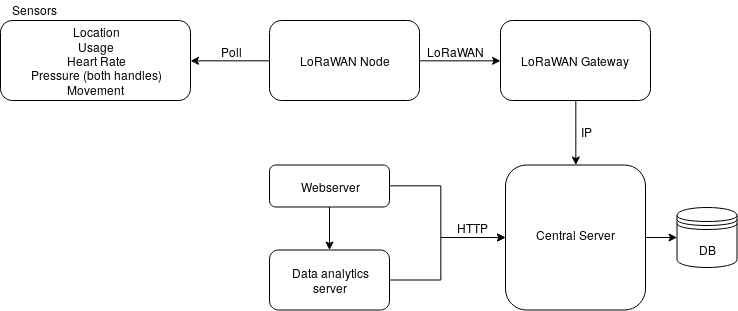
\includegraphics[width=0.7\linewidth]{gfx/image1}
\caption{Proposed architecture}
\label{fig:image1}
\end{figure}

Based on our proposed architecture, we can summarize the components and their functionalities as follows:

\begin{center}
\begin{tabular}{|c|c|}
\hline
Component	& Function \\ 
\hline
Walker	&  Helps user walk\\ 
LoRaWAN Node	& Collects and sends param \\ 
Sensors		& Extracts user/walker info \\ 
LoRaWAN Gateway	& Relays LoRaWAN packets  \\ 
Server	& Receives and stores data \\
\hline

\end{tabular} 

\end{center}

The proposed architecture can be realized in a number of ways, meaning we had to make the following choices:
\begin{itemize}
	\item Use sensors with inbuilt LoRa functionality or use a single-board computer connected to sensors and LoRa transmitter ?
	\item What hardware to use to interface with the sensors and act as the node ?
	\item What hardware to use as LoRaWAN gateway ?
\end{itemize}



\subsection{Single-board Computer vs Inbuilt LoRa Sensors:}

We had the option of using a single-board computer (SBC) to interface with all of the sensors (Arduino or Rpi) or using sensors with inbuilt LoRaWAN capabilities.

We summarized the haracteristics of sensors with inbuilt LoRaWAN as follows:
\begin{itemize}
	\item They require little to no configuration and work out of the box. This means using them would grant us more time to we can focus on other parts of the project.
	\item Data can be sent at different rates for each sensor.
	\item They are much more expensive than standard sensors.
	\item They are bulkier than standard sensors, making them harder to fit into the walker.
	\item Their is low variety when it comes to such sensors in the market, limiting choice of vendor and sensors.
	\item Having several LoRaWAN transmitters instead of one would make the power consumption higher.
\end{itemize}


We summarized the following characteristics of SBCs:
\begin{itemize}
	\item Fine grained control of the sensors
	\item We might want to do some preprocessing of the sensor data before sending it, which is possible with SBCs.
	\item Good amount of variety in the market allowing us a lot of choice.
\end{itemize}

We decided to go with an SBC because we value the flexibility provided by the vast array of sensors to choose from and the possibility to manually program them.



\subsection{Comparing Raspberry Pi and Arduino:}

We then had the option of either using a Raspberry Pi or an Arduino. We summarized their characteristics as follows:

Pi:
\begin{itemize}
	\item Faster and more powerful processor
	\item Overhead of operating system, hdmi output, wifi/ethernet port, audio output, all of which take physical or disk space.
	\item More power consumption
\end{itemize}

Arduino:
\begin{itemize}
	\item Easy to get up and running
	\item Easier to connect with analog sensors
	\item Lots of different models to choose from, meaning we can choose the one that best fits our goals
	\item Cheaper than the Raspberry Pi
	\item Smaller 
	\item No operating system, meaning we are closer to the hardware and have more control over the sensors
\end{itemize}



Due to the points mentioned above, especially due to its flexibility, and low power consumption, we decided to go with the arduino as the node.

Due to its superior computational power, inbuilt networking capabilities, we decided to go with the Raspberry Pi as the gateway.

Our reasoning is supported by the arguments put forward in \cite{postolache2011smart}.


\subsection{Experiments:}
In order to test our hypothesis, we designed the following experiments:

\subsubsection{Feasibility:}
In order to consider our hypothesis feasible we need to have some data being collected from sensors attached to a walker and sent through LoRaWAN to a remote server.

\subsubsection{Consistency:}
To test consistency we will devise some usage scenarios and for each of them get 10 measurements. We will then compare the precision within and between scenarios by getting the variance.

\subsubsection{Accuracy:}
In order to measure accuracy we need to find the difference between the measured value of each sensor and compare it to the true value. This means we need a test tailored to each sensor. For this, we will perform 10 measurements from each sensor after performing identical displacement or task and then find standard deviation of the measured values from the true value.

\subsubsection{Reliability:}
To measure reliability we will use the walker until we get 20 measurements and calculate the percentage of times they got stored in the server’s database


\subsubsection{Durability:}
Unfortunately, we don’t have enough time to test the durability of our system, so we’ll leave this as a possible improvement over our project



\subsubsection{Modularity:}
In order to test the modularity of the system, we will deliberately only integrate the GPS sensor in the testing phase of the project, this way we can measure how much time it takes and analyse the complications brought by doing so.

\subsubsection{Scalability:}
With the resources at our disposal, we will, additionally to the walker, have another node collecting pressure data and sending it through our system. If both of the node’s data get safely stored in the server, we can be confident that our system supports at least two walkers

\subsubsection{Serviceability:}
One of the members of the team will disconnect random cables connecting the sensors to the node and we will then have another member get the system back up and running while measuring the time it took


%%% Local Variables:
%%% mode: latex
%%% TeX-master: "../ClassicThesis"
%%% End:
